%%%%%%%%%%%%%%%%%%%%%%%%%%%%%%%%%%%%%%%%%
% Masters/Doctoral Thesis 
% LaTeX Template
% Version 1.43 (17/5/14)
%
% This template has been downloaded from:
% http://www.LaTeXTemplates.com
%
% Original authors:
% Steven Gunn 
% http://users.ecs.soton.ac.uk/srg/softwaretools/document/templates/
% and
% Sunil Patel
% http://www.sunilpatel.co.uk/thesis-template/
%
% License:
% CC BY-NC-SA 3.0 (http://creativecommons.org/licenses/by-nc-sa/3.0/)
%
% Note:
% Make sure to edit document variables in the Thesis.cls file
%
%%%%%%%%%%%%%%%%%%%%%%%%%%%%%%%%%%%%%%%%%

%----------------------------------------------------------------------------------------
%	PACKAGES AND OTHER DOCUMENT CONFIGURATIONS
%----------------------------------------------------------------------------------------

\documentclass[11pt, oneside]{Thesis} % The default font size and one-sided printing (no margin offsets)

\graphicspath{{Pictures/}} % Specifies the directory where pictures are stored
\usepackage[square, numbers, comma, sort&compress]{natbib} 
\usepackage{csvsimple}
% Use the natbib reference package - read up on this to edit the reference style; 
% if you want text (e.g. Smith et al., 2012) for the in-text references (instead of numbers), remove %'numbers' 

\hypersetup{urlcolor=blue, colorlinks=true} % Colors hyperlinks in blue - change to black if annoying
\title{\ttitle} % Defines the thesis title - don't touch this
\begin{document}

\frontmatter % Use roman page numbering style (i, ii, iii, iv...) for the pre-content pages

\setstretch{1.3} % Line spacing of 1.3

% Define the page headers using the FancyHdr package and set up for one-sided printing
\fancyhead{} % Clears all page headers and footers
\rhead{\thepage} % Sets the right side header to show the page number
\lhead{} % Clears the left side page header

\pagestyle{fancy} % Finally, use the "fancy" page style to implement the FancyHdr headers

\newcommand{\HRule}{\rule{\linewidth}{0.5mm}} % New command to make the lines in the title page

% PDF meta-datar
\hypersetup{pdftitle={\ttitle}}
\hypersetup{pdfsubject=\subjectname}
\hypersetup{pdfauthor=\authornames}
\hypersetup{pdfkeywords=\keywordnames}

%----------------------------------------------------------------------------------------
%	TITLE PAGE
%----------------------------------------------------------------------------------------

\begin{titlepage}
\begin{center}

\textsc{\LARGE \univname}\\[1.5cm] % University name
\textsc{\Large Tesi Di Laurea Triennale}\\[0.5cm] % Thesis type

\HRule \\[0.4cm] % Horizontal line
{\huge \bfseries \ttitle}\\[0.4cm] % Thesis title
\HRule \\[1.5cm] % Horizontal line
 
\begin{minipage}{0.4\textwidth}

\begin{flushleft} \large
\emph{Author:}\\
\authornames             % Author name - remove the \href bracket to remove the link
\end{flushleft}
\end{minipage}
\begin{minipage}{0.4\textwidth}
\begin{flushright} \large
\emph{Relatore:} \\
\supname		 % Supervisor name - remove the \href bracket to remove the link

\emph{Correlatore:} \\
\cosupname		 % Cosupervisor name -
\end{flushright}
\end{minipage}\\[3cm]
 
%\large \textit{A thesis submitted in fulfilment of the requirements\\ for the degree of \degreename}\\[0.3cm] % University requirement text
%\textit{in the}\\[0.4cm]
\deptname\\[2cm] % Research group name and department name
 
{\large \today}\\[4cm] % Date
%\includegraphics{Logo} % University/department logo - uncomment to place it
 
\vfill
\end{center}

\end{titlepage}
  

\clearpage % Start a new page

%----------------------------------------------------------------------------------------
%	QUOTATION PAGE
%----------------------------------------------------------------------------------------

\pagestyle{empty} % No headers or footers for the following pages

\null\vfill % Add some space to move the quote down the page a bit

\textit{``textfit``}

\begin{flushright}
-
\end{flushright}

\vfill
\vfill
\vfill

\vfill
\vfill
\vfill
\vfill
\null % Add some space at the bottom to position the quote just right

\clearpage % Start a new page

%----------------------------------------------------------------------------------------
%	ABSTRACT PAGE -- see the design on Thesis.cls
%----------------------------------------------------------------------------------------

\addtotoc{Abstract} % Add the "Abstract" page entry to the Contents

\abstract{\addtocontents{toc}{\vspace{1em}} % Add a gap in the Contents, for aesthetics
I dispositivi mobili, al giorno d’oggi, rivestono un ruolo sempre più importante tanto nelle aziende quando nella nostra vita privata, permettendoci di compiere operazioni e svolgere dei compiti che, fino a qualche anno fa, erano eseguibili solo attraverso un normale PC.
Con il passare del tempo, l’evoluzione tecnologica che ha accompagnato lo sviluppo dei normali PC, ha coinvolto i dispositivi così detti “mobili”. Evoluzione che li ha trasformati da semplici organizer “da tasca” a veri e propri terminali ricchi di funzionalità, discreta potenza di calcolo ma soprattutto di connettività. Quest’ultima caratteristica li ha resi estremamente versatili soprattutto per applicazioni di tipo aziendale e di produttività personale.

\textit{Dai dati sull’uso dei differenti device utilizzati per accedere a internet, risulta che il 66,4\% del tempo totale speso online è generato dalla fruizione di internet da mobile e, più in dettaglio, il 	55,7\% del totale dalla fruizione tramite mobile applications.}

\textit{Fonte Audiweb Database, Agosto 2014}

Il nostro compito, in quanto sviluppatori, è quello di realizzare applicazioni non solo funzionanti nel senso stretto del termine ma funzionali e usabili su questa tipologia di dispositivi. Inoltre se vogliamo far conoscere il nostro prodotto ad un numero maggiore di utenti, dobbiamo anche preoccuparci che la nostra applicazione sia disponibile su diverse piattaforme, perché come ben sappiamo il mercato dei dispositivi mobili ha diversi sistemi operativi su cui possiamo sviluppare, ed ognuno di essi usa modelli e linguaggi di programmazione differenti.

Esistono diversi modi per sviluppare una applicazione mobile, Nativa, Web o ibrida: Non esiste la risposta perfetta. Tutte hanno vantaggi e svantaggi e la scelta può limitare le opzioni degli strumenti di sviluppo in un secondo momento.

\paragraph*{App native} Sviluppare un'app utilizzando l'interfaccia e il linguaggio di programmazione per un determinato dispositivo e sistema operativo. Ciò può fornire le prestazioni migliori ma richiede una versione differente (costosa) per ogni sistema operativo.

\paragraph*{App Web} Molti nuovi dispositivi utilizzano un browser per fornire un aspetto tradizionale alle app mobile. Ciò consente di supportare molti dispositivi ma spesso non offre l'accesso alle funzioni dei dispositivi mobile, come la fotocamera o l'elenco dei contatti.

\paragraph*{App ibride} Un compromesso tra nativa e Web. Lo sviluppo avviene utilizzando i linguaggi di programmazione Web standard di settore, come HTML5 e JavaScript quindi viene creato un pacchetto di installazione nativa (es. apk file) per la distribuzione tramite app store. E' cosi possibile ridurre i costi con il riutilizzo del codice.

L'obiettivo di questo lavoro e quello di trovare un metodo di sviluppo veloce per avere la stessa applicazione disponibile nelle diverse piattaforme. Ovviamente ci sono più percorsi che ci possono portare allo stesso risultato, la scelta della strada intrapresa dipende dalle conoscenze iniziali dello sviluppatore. 

Questa tesi si propone l'obiettivo di analizzare le tecnologie sul mercato attuale e proporre un modello di sviluppo rapido di applicazioni multi-piattaforma per dispositivi mobili, attraverso l'utilizzo di tecnologie web.

}

\clearpage % Start a new page

%----------------------------------------------------------------------------------------
%	ACKNOWLEDGEMENTS
%----------------------------------------------------------------------------------------

\setstretch{1.3} % Reset the line-spacing to 1.3 for body text (if it has changed)

\acknowledgements{\addtocontents{toc}{\vspace{1em}} % Add a gap in the Contents, for aesthetics

Grazie a tutti \ldots
}
\clearpage % Start a new page

%----------------------------------------------------------------------------------------
%	LIST OF CONTENTS/FIGURES/TABLES PAGES
%----------------------------------------------------------------------------------------

\pagestyle{fancy} % The page style headers have been "empty" all this time, now use the "fancy" headers as defined before to bring them back

\lhead{\emph{Contents}} % Set the left side page header to "Contents"
\tableofcontents % Write out the Table of Contents

\lhead{\emph{List of Figures}} % Set the left side page header to "List of Figures"
\listoffigures % Write out the List of Figures

\lhead{\emph{List of Tables}} % Set the left side page header to "List of Tables"
\listoftables % Write out the List of Tables

%----------------------------------------------------------------------------------------
%	ABBREVIATIONS
%----------------------------------------------------------------------------------------

%\clearpage % Start a new page

%\setstretch{1.5} % Set the line spacing to 1.5, this makes the following tables easier to read

%\lhead{\emph{Abbreviations}} % Set the left side page header to "Abbreviations"
%\listofsymbols{ll} % Include a list of Abbreviations (a table of two columns)
%{
%\textbf{ASAP} & \textbf{A}s \textbf{S}oon \textbf{A}s \textbf{P}ossible \\
%\textbf{HTML} & \textbf{H}yper\textbf{T}ext \textbf{M}arkup \textbf{L}anguage \\
%\textbf{CSS} & \textbf{C}ascading \textbf{S}tyle \textbf{S}heet \\
%\textbf{RIA} & \textbf{R}ich \textbf{I}nternet \textbf{A}pplication \\
%\textbf{Acronym} & \textbf{W}hat (it) \textbf{S}tands \textbf{F}or \\
%}

%----------------------------------------------------------------------------------------
%	PHYSICAL CONSTANTS/OTHER DEFINITIONS
%----------------------------------------------------------------------------------------

%\clearpage % Start a new page

%\lhead{\emph{Physical Constants}} % Set the left side page header to "Physical Constants"

%\listofconstants{lrcl} % Include a list of Physical Constants (a four column table)
%{
%Speed of Light & $c$ & $=$ & $2.997\ 924\ 58\times10^{8}\ \mbox{ms}^{-\mbox{s}}$ (exact)\\
% Constant Name & Symbol & = & Constant Value (with units) \\
%}

%----------------------------------------------------------------------------------------
%	SYMBOLS
%----------------------------------------------------------------------------------------

%\clearpage % Start a new page

%\lhead{\emph{Symbols}} % Set the left side page header to "Symbols"

%\listofnomenclature{lll} % Include a list of Symbols (a three column table)
%{
%$a$ & distance & m \\
%$P$ & power & W (Js$^{-1}$) \\
% Symbol & Name & Unit \\

%& & \\ % Gap to separate the Roman symbols from the Greek

%$\omega$ & angular frequency & rads$^{-1}$ \\
% Symbol & Name & Unit \\
%}

%----------------------------------------------------------------------------------------
%	DEDICATION
%----------------------------------------------------------------------------------------

\setstretch{1.3} % Return the line spacing back to 1.3

\pagestyle{empty} % Page style needs to be empty for this page

\dedicatory{For/Dedicated to/To my\ldots} % Dedication text

\addtocontents{toc}{\vspace{2em}} % Add a gap in the Contents, for aesthetics

%----------------------------------------------------------------------------------------
%	THESIS CONTENT - CHAPTERS
%----------------------------------------------------------------------------------------

\mainmatter % Begin numeric (1,2,3...) page numbering

\pagestyle{fancy} % Return the page headers back to the "fancy" style

% Include the chapters of the thesis as separate files from the Chapters folder
% Uncomment the lines as you write the chapters

\lhead{\emph{Capitolo 1}}
\chapter{Stato dell'arte} 
In questo capitolo si presentano le tecnologie attualmente presenti sul mercato per lo sviluppo di applicazioni mobili, con particolare attenzione per le strategie di sviluppo multi piattaforma.
\section{Sviluppo Nativo}
Nello sviluppo nativo ogni applicazione viene sviluppata singolarmente per ogni piattaforma; rispettivamente per ogni sistema operativo bisogna conoscere i linguaggi che vengono utilizzati.

\csvautotabular{Primitives/platforms.csv}

Il punto di forza che ha questo tipo di approccio sta sicuramente nelle prestazioni dell'applicazione e nel completo accesso a tutte le possibilità del nostro dispositivo. Tuttavia con questo tipo sviluppo richiede molto tempo nel caso della distribuzione su più piattaforme.
\section{Multi-Piattaforma}

\subsection{Web Applications}
Quando si intraprende la strada dello sviluppo di una applicazione multi-piattaforma l'opzione più semplice è sicuramente quella di creare una Web App responsive\footnote{indica la capacità di una Web App o di un sito internet di adattare le proprie dimensioni e proporzioni in base alla risoluzione del dispositivo con il quale vengono visualizzati} che sia accessibile in modo immediato dal browser web del nostro dispositivo. In questo caso i tempi di sviluppo sono veramente esigui, e non abbiamo bisogno di aggiornamenti in quanto si tratta alla fine di un piccolo sito internet(quindi ci basta aggiornare la pagina).

A scapito della velocità di produzione e della facilità di aggiornamento non possiamo permetterci alcune caratteristiche fondamentali per le applicazioni mobile, come ad esempio accedere alle funzionalità del nostro dispositivo come fotocamera o rubrica, oppure memorizzare dati sul nostro dispositivo(o meglio possiamo farlo ma sfruttando solamente la cache del browser web) ma la criticità maggiore sta nel fatto che la connessione internet deve essere sempre presente. 

\subsection{I Framework}
L'approccio ibrido che si propone combina la velocità di sviluppo delle Web App con un accesso \emph{quasi nativo} al nostro dispositivo. Un problema che ci so pone in questo tipo di approccio sta nella scelta del \emph{framework} che si adatta  meglio allo scopo della nostra applicazione.

\textit{In informatica, e specificatamente nello sviluppo software, un \textbf{framework} è un'architettura (o più impropriamente struttura) logica di supporto (spesso un'implementazione logica di un particolare design pattern) su cui un software può essere progettato e realizzato, spesso facilitandone lo sviluppo da parte del programmatore. Alla base di un framework c'è sempre una serie di librerie di codice utilizzabili in fase di linking con uno o più linguaggi di programmazione, spesso corredate da una serie di strumenti di supporto allo sviluppo del software, come ad esempio un IDE, un debugger o altri strumenti ideati per aumentare la velocità di sviluppo del prodotto finito. L'utilizzo di un framework impone dunque al programmatore una precisa metodologia di sviluppo del software.}\\
\hspace*{\fill}\citeauthor{wiki:framework}

Esistono diversi framework sul mercato con caratteristiche diverse tra di loro, ecco quelli più popolari:

\csvautotabular{Primitives/frameworks.csv}

Ogni framework adotta strategie diverse per passare dal codice sorgente a quello di destinazione, successivamente verranno discusse alcune di esse.

\subsubsection{Wrapper}
I framework denominati appunto \texttt{Wrapper} sfruttano il design pattern strutturale \texttt{Adapter} e operano quindi una astrazione sul linguaggio di destinazione. In questo caso il framework ha il compito di intermediario tra il linguaggio usato nella applicazione e quello nativo del dispositivo.
Cordova ad esempio simula un browser web sul linguaggio di astrazione(che in questo caso saranno linguaggi in ambito web) e fornisce delle API per comunicare con la parte nativa del linguaggio del dispositivo.
La game-engine \texttt{Unity} utilizza lo stesso meccanismo si astrazione, ed anziché simulare un browser utilizza un linguaggio proprietario per poter eseguire la applicazione su più piattaforme.
Un altro esempio è invece Apache Flex che utilizza come linguaggio di astrazione Adobe Flash e in alcuni casi Javascript.
\subsubsection{Trasformazione del Codice}
Alcuni framework potremmo definirli invece \emph{"trasformatori"} ovvero partendo da un loro linguaggio / metalinguaggio(spesso somigliante ad altri linguaggi conosciuti come ad esempio Java) producono un il codice specifico per ogni sistema operativo scelto.
In particolare il linguaggio utilizzato dal framework è una associazione tra il suo linguaggio è quello di destinazione. Una volta creata e riconosciuta l'associazione, il codice viene trasformato.
\subsubsection{User Interface}
Altri tipi di framework invece sono atti alla definizione dell'interfaccia utente della nostra applicazione, ovvero si traducono in un insieme di librerie che utilizzano metalinguaggi e non per \emph{"vestire"} la nostra applicazione a seconda dello scopo.
Un esempio di un framework di questo tipo è \texttt{Ionic}, il quale fornisce un set di stili e funzioni per la nostra applicazione utilizzando tecnologie web, come ad esempio menù laterali, bottoni, form, icone. La maggior parte di questi tipi di framework fornisce anche linee guida per creare elementi completamente nuovi, nel caso avessimo bisogno di parti più complesse.
Invece \texttt{Apache Flex}, oltre a fungere da wrapper, fornisce un set di elementi già pronti e parametrizzati (il linguaggio è simile a XML\footnote{(sigla di eXtensible Markup Language) è un linguaggio di markup, ovvero un linguaggio marcatore basato su un meccanismo sintattico che consente di definire e controllare il significato degli elementi contenuti in un documento o in un testo.\citeauthor{wiki:xml}}) per poter personalizzare la nostra applicazione. Non è molto versatile ma è particolarmente adatto alle applicazioni nel campo produttivo/finanziario.
\section{Vantaggi e Svantaggi}
Il vantaggio principale nell’utilizzo di un framework consiste nella possibilità di effettuare un deploy rapido e multipiattaforma di un’applicazione: il codice, infatti, si scrive velocemente con un meta linguaggio ed attraverso librerie esistenti precompilate, ed esso viene automaticamente adattato per i diversi sistemi operativi in fase di compilazione.

Un limite dei framework consiste nell’eccesso di rigidità in fase progettuale: il loro utilizzo, infatti, limita in parte la possibilità di sfruttare le caratteristiche native del device, delle linee guida dell’interfaccia e del sistema operativo che utilizzerà l’applicazione, e spesso, quindi, si corre il rischio di non riuscire a sviluppare interfacce utente pienamente ergonomiche e intuitive.
Inoltre, alcuni framework sono più adatti ad impieghi specifici rispetto ad altri. Kony, ad esempio, è un tipo di framework particolarmente apprezzato nello sviluppo di applicazioni per il settore bancario e financial, poichè integra al suo interno numerose funzioni utili,tra cui per la gestione dei sistemi di pagamento attraverso gli smartphone.

Un tipo di framework scelto nel contesto giusto, che tenga concretamente conto degli obiettivi di marketing dell’azienda e le strategie di investimento in sviluppo di prodotti, consente di ottimizzare i tempi di sviluppo, presentare velocemente sul mercato la propria applicazione ed ottimizzare il processo di delivery abbattendo costi e sfruttando le potenzialità specifiche del framework selezionato.\\
\hspace*{\fill}\citep{web:framework}


% Chapter Template

\chapter{HTML, CSS, Javascript - L'evoluzione dei linguaggi web} % Main chapter title

\label{ChapterX} % Change X to a consecutive number; for referencing this chapter elsewhere, use \ref{ChapterX}

\lhead{Chapter X. \emph{Chapter Title Here}} % Change X to a consecutive number; this is for the header on each page - perhaps a shortened title

Linguaggi come l'HTML(Hypertext Markup Language), CSS(Cascading Style Sheet) e Javascript sono i principali strumenti con quali costruiamo pagine web, ebbene la continua evoluzione di questi linguaggi ha portato il classico sito web, a somigliare molto ad una applicazione vera e propria. 
Questo però non sarebbe stato possible se  questi tre linguaggi on si fosssero evoluti parallelamente.
\section{L'HTML - Da descrittore di documenti a descrittore di interfacce}


\section{CSS - Dallo stile dei documenti alle trasformazioni vettoriali}


\section{Javascript - Dalle animazioni ai potenti Framework}
Morbi rutrum odio eget arcu adipiscing sodales. Aenean et purus a est pulvinar pellentesque. Cras in elit neque, quis varius elit. Phasellus fringilla, nibh eu tempus venenatis, dolor elit posuere quam, quis adipiscing urna leo nec orci. Sed nec nulla auctor odio aliquet consequat. Ut nec nulla in ante ullamcorper aliquam at sed dolor. Phasellus fermentum magna in augue gravida cursus. Cras sed pretium lorem. Pellentesque eget ornare odio. Proin accumsan, massa viverra cursus pharetra, ipsum nisi lobortis velit, a malesuada dolor lorem eu neque.

%----------------------------------------------------------------------------------------
%	SECTION 2
%----------------------------------------------------------------------------------------

\section{Main Section 2}

Sed ullamcorper quam eu nisl interdum at interdum enim egestas. Aliquam placerat justo sed lectus lobortis ut porta nisl porttitor. Vestibulum mi dolor, lacinia molestie gravida at, tempus vitae ligula. Donec eget quam sapien, in viverra eros. Donec pellentesque justo a massa fringilla non vestibulum metus vestibulum. Vestibulum in orci quis felis tempor lacinia. Vivamus ornare ultrices facilisis. Ut hendrerit volutpat vulputate. Morbi condimentum venenatis augue, id porta ipsum vulputate in. Curabitur luctus tempus justo. Vestibulum risus lectus, adipiscing nec condimentum quis, condimentum nec nisl. Aliquam dictum sagittis velit sed iaculis. Morbi tristique augue sit amet nulla pulvinar id facilisis ligula mollis. Nam elit libero, tincidunt ut aliquam at, molestie in quam. Aenean rhoncus vehicula hendrerit. 
\lhead{\emph{Capitolo 3}}
\chapter{Case Study: L'approccio ibrido con tecnologie web}

L'approccio ibrido con tecnologie web è stato scelto durante lo svolgimento del tirocinio presso la ditta BigThink SRL, in quanto si adattava meglio ad una serie di tecnologie già utilizzate dall'azienda.
Durante la permanenza in azienda ho svolto il lavoro di Frontend Developer di Web Applications, in particolare mi occupavo dello sviluppo della logica di business di una applicazione e della sua interfaccia.
Una delle politiche dell'azienda era quella di separare la gestione dei dati e la loro memorizzazione lato Backend in modo tale che la parte Frontend sviluppata con il framework Javascript AngularJS si interfacciasse con i dati servendosi solo di API REST.
Data il numero consistente di Web Application sviluppate e il mercato di applicazioni Mobile sempre in crescita, sono stato incaricato dall'azienda di ricercare dei metodi e delle tecnologie che consentissero di portare il lavoro già fatto per le Web Application su dispositivo mobili, in modo tale che l'azienda avesse nuovi servizi da offrire.\\
Tutte le applicazioni sviluppate fino ad allora erano già Responsive Web Application, in azienda si volevano aggiungere funzionalità caratteristiche dei dispositivi mobili tramite l'utilizzo di tecnologie web.\\

Un primo punto di riferimento come tecnologia Web è stato AgnularJS, framework già utilizzato dall'azienda, se fosse stato scelto un altro framework si sarebbe dovuto riscrivere tutto il codice delle Web Application già sviluppate fino a quel punto. A questo punto  si trattava di scegliere le corrette tecnologie per includere al meglio il lavoro già svolto, in particolare un Wrapper che avrebbe consentito un buon sviluppo dell'applicazione partendo da tecnologie web, senza influire su eventuali spese aziendali. 

Per quanto riguarda gli strumenti di sviluppo utilizzati la scelta rimane allo sviluppatore, nel mio caso ho preferito elencarne alcuni secondo me importanti utilizzati all'interno dell'azienda e scoperti durante l'attività di ricerca.

\section{Le Tecnologie Web utilizzate}
Il riferimento per la scelta di tecnologie web è stato il framework AngularJS, il quale è utilizzato a sua volta all'interno di altri framework, come ad esempio Ionic che fornisce degli strumenti per la creazione di interfacce utente. Come Wrapper ho scelto Cordova, in quanto oltre ad essere un progetto open-source fornisce delle API per le funzionalità del dispositivo in linguaggio Javascript. Inoltre esiste un'ultima libreria che richiama le funzionalità di Cordova utilizzando il framwork AngularJS, il che viene molto comodo per il set di tecnologie scelto.

Il framework Ionic per la creazione dell'interfaccia utente è composto oltre da AngularJS da altre tecnologie come un \emph{CSS Preprocessor} che verrà spiegato prima di introdurre nel dettaglio le tencnologie introdotte precedentemente.

\subsection{CSS Preprocessor}

Nei Web Framework che forniscono strumenti per la definizione di interfacce utente un componente che si trova molto spesso e il \emph{CSS Preporcessor} ovvero un preprocessore di fogli di stile.

\emph{In informatica, un preprocessore o precompilatore è un programma (o una porzione di programma) che effettua sostituzioni testuali sul codice sorgente di un programma, ovvero la precompilazione. I più comuni tipi di sostituzioni sono l'espansione di macro, l'inclusione di altri file, e la compilazione condizionale (vedi conditional compilation in inglese). Tipicamente, il preprocessore viene lanciato nel processo di compilazione di un software, e il file risultante verrà preso in input da un compilatore.}
\hspace*{\fill}\cite{wiki:preprocessor} 

\begin{figure}[htbp]
  \centering
    
\includegraphics[scale=0.25]{Figures/sass-logo.png} 
    
\includegraphics[scale=0.75]{Figures/less-logo.png} 
    \rule{35em}{0.5pt}
  \caption[Css Preprocessors]{\textbf{S}intatically \textbf{A}wesome \textbf{S}tyle\textbf{S}heet e \textbf{LESS}}
  \label{fig:CSS Preprocessors}
\end{figure}



Essendo CSS un linguaggio fortemente dichiarativo basato sui markup HTML, fa si che i fogli di stile per interfacce utente diventino molto lunghi e verbosi data la complessità. E di conseguenza la personalizzazione da parte dello sviluppatore che andrà a utilizzare il framework diventa molto difficile.
I CSS preprocessor mettono a disposizione un set di operazioni chiamate MACRO che durante la compilazione verranno sostituite con il linguaggio CSS prorpio. Queste MACRO consentono ad esempio di fare utilizzo di variabili, funzioni, tag parametrici, ereditarietà dei tag, pattern matching, namespaces.

Queste sono solo alcune delle opzioni messe a disposizione dei CSS preprocessors dipende dalle sviluppatore scegliere quello secondo lui più adatto in quanto sul mercato ne esistono diversi, i più famosi e utilizzati sono \textbf{SASS}(\textbf{S}intatically \textbf{A}wesome \textbf{S}tyle\textbf{S}heet) e \textbf{LESS}(write \textbf{LESS} do more) \ref{fig:CSS Preprocessors}.

\subsection{AngularJS}

\begin{wrapfigure}{r}{0.40\textwidth}
  \vspace{-65pt}
  \begin{center}
    
\includegraphics[scale=0.40]{Figures/angular-logo.png}
  \end{center}
  \vspace{-10pt}
  \caption{\\AngularJS framework logo}
  \label{fig:AngularJS}
  \vspace{10pt}
\end{wrapfigure}

\paragraph{Definizione}
AngularJS è un framework Javascript ideato da \emph{Minsko Hevery}(Google) che estende il linguaggio HTML in un formato più espressivo e leggibile. Consente di aggiungere nuovi tag HTML speciali in modo da sincronizzare la parte scritta in Javascript senza manualmente aggiornare la view, in modo tale da rendere indipendente la logica della applicazione. Angular semplifica la scrittura di codice Javascript rendendo il codice dell'applicazione più efficiente e leggibile.
\paragraph{Caratteristiche e Componenti}
AngularJS interpreta il design pattern MVC grazie al quale si arricchisce con una serie di caratteristiche molto interessanti:
\begin{description}

\item[Data Binding] Il Data Binding in AngularJS è la sincronizzazione automatica dei dati tra modello e vista. In modo in cui AngularJS implementa il data bindign consente di trattare il modello come SSOT(\cite{wiki:SSOT}). La vista è la proiezione del modello in ogni momento, quando il modello cambia la vista riflette il cambiamento e viceversa. 
La maggior parte dei sistemi di templating sincronizzano i dati in una sola direzione: si fondono componenti del template e modello insieme in una vista. Quando si verifica la fusione, le modifiche al modello o sezioni correlate della vista vengono NON si riflettono automaticamente nella vista. Peggio ancora, le eventuali modifiche che l'utente fa nella vista non si riflettono nel modello. Ciò significa che lo sviluppatore deve scrivere del codice apposito che sincronizza costantemente la vista con il modello e il modello con la vista.

\begin{figure}[htbp]
  \centering
    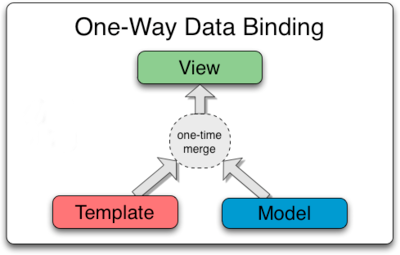
\includegraphics[scale=0.5]{Figures/one-way-data-binding.png} 
    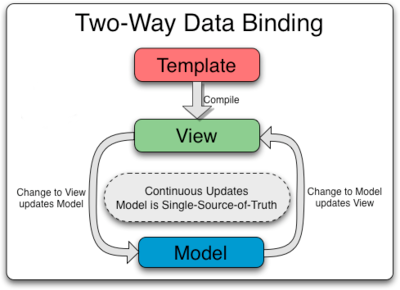
\includegraphics[scale=0.5]{Figures/two-way-data-binding.png} 
    \rule{35em}{0.5pt}
  \caption[Data Bindings]{Come è strutturato un classico data binding, e come invece è fatto in AngularJS}
  \label{fig:Data Binding}
\end{figure}

Il systema dei templates di AngularJS funziona in modo differente. In primo luogo il modello (che è l'HTML non compilato insieme a  markup o direttive supplementari) viene compilato sul browser. Il passo di compilazione produce una live view(vista). Eventuali modifiche alla vista si riflettono immediatamente nel modello, e le eventuali modifiche nel modello vengono propagate alla vista. Il modello è il SSOT per lo stato dell'applicazione, semplificando notevolmente il modello di programmazione per lo sviluppatore. Si può pensare di vista semplicemente come una proiezione istantanea del modello.

Poiché la vista è solo una proiezione del modello, il controller è completamente separato dal punto di vista e completamente allo scuro di essa. Questo rende i test dell'applicazione molto semplici, in quanto è facile testare il controller indipendentemente dalla vista e dalla relativa dipendenza dal DOM / browser web.

\item[Scope] Lo \emph{Scope} è un oggetto che si riferisce al modello dell'applicazione. E' il contesto dove vengono eseguite le espressioni. Esistono più scope all'interno dell'applicazione e sono organizzati in maniera gerarchica ad imitare la struttura del DOM dell'applicazione. Infine sullo scope si può osservare una espressione e propagare eventi.
I vari scope di una applicazione in AngularJS sono i nodi centrali a cui ruota attorno tutta la logica dell'applicazione, grazie a loro e possibile la comunicazione tra vista e modello con l'utilizzo del data binding. Per una trattazione più approfondita si rimanda alla documentazione di AngularJS(angularjs.org).

\item[Controller] i controller in AngularJS hanno il compito di gestire la logica di una determinata sezione dell'applicazione. Quando un controller viene dichiarato su una parte del DOM tramite la direttiva \emph{ng-controller} come nell'esempio \ref{lst:newController} AngularJS crea un nuovo oggetto Javascript associandogli un nuovo scope che potrà essere inserito all'interno del controller tramite la dependency injection. 
\clearpage
\begin{lstlisting}[caption={Associazione tra un elemento del DOM e un controller}, label={lst:newController}]
	<div id="header" ng-controller = "HeaderController"></div>
\end{lstlisting}
In generale ci sono alcune regole da seguire per la creazione dei controller, le quali non sono obbligatorie ma sono considerate come si dice in gergo \emph{Best Practices}:
I controller devono essere usati per:
\begin{itemize}
\item Configurare lo stato iniziale dello scope.
\item Aggiungere comportamento allo scope(funzioni, modelli, oggetti)
\end{itemize}
Mentre i controller non devono essere usati per:
\begin{itemize}
\item Manipolare elementi del DOM
\item Formattare input e output
\item Condividere codice tra i vari controller.
\item Gestire il ciclo di vita degli altri componenti(creazione di nuove istanze)
\end{itemize}

\item[Dependency Injection] per una trattazione generale dell'argomento rimandiamo all'appendice \ref{app:DepInj}. In AngularJS è definito un Injector Subsystem che ha l'incarico di creare i componenti, risolvere le loro dipendenze e fornire i componenti richiesti. 

\end{description} 
	-- MVC --	
	-- Dependency Injection --\\
	-- Moduli --\\
	-- View --\\
	-- Factory --\\
	-- Directives --\\
	-- Filters --\\

\subsection{Ionic}

\begin{wrapfigure}{r}{0.40\textwidth}
  \vspace{-65pt}
  \begin{center}
    
\includegraphics[scale=0.35]{Figures/ionic-logo.png}
  \end{center}
  \vspace{-10pt}
  \caption{Ionic Framework Logo}
  \label{fig:IONIC}
  \vspace{5pt}
\end{wrapfigure}

Ionic offre componenti e librerie pensati per uno sviluppo ibrido dell'applicazione, inoltre è stato sviluppato riducendo al minimo la manipolazione del DOM\footnote{Il Document Object Model (spesso abbreviato come DOM), letteralmente modello a oggetti del documento, è una forma di rappresentazione dei documenti strutturati come modello orientato agli oggetti.\cite{wiki:dom} gli oggetti delle pagine web, ad esempio con delle animazioni, introduciamo della computazione aggiuntiva al nostro browser che può rallentarne le prestazioni} garantendo performance molto competitive.\\
I componenti di Ionic vengono ovviamente strutturati tramite HTML5, aggiungendo classi css specifiche del framework. Inoltre 
Ionic fornisce uno strumento molto interessante da linea di comando che permette di scaricare diversi modelli di applicazione già pronti in modo da non dover tutte le volte configurare da capo la nostra applicazione con il framework. Inoltre ci predispone i file in una maniera logica ben precisa cosicché se volessimo in un futuro aggiungere codice e/o altre librerie possiamo farlo con molta facilità.
I componenti non sono altro che elementi del linguaggio HTML, vengono forniti con una serie di classi CSS caratteristiche del framework, pensate in modo da essere componibili tra di loro. Ionic fornisce inoltre dei tag propri del framework che possono includere elementi più complessi come ad esempio menù laterali.
Il cuore di Ionic e tutte le sue funzionlità sono state sviluppate in AngularJS il che rende questo framework ancora più versatile e potente. Inoltre tutti il foglio di stile che include Ionic fa uso di SASS e ci da la possibilità di personalizzare colori e forme dei componenti semplicemente ricompilando i file \emph{.scss}.
\section{Il Wrapper Framework}

- Perche ho scelto un wrapper \\
	-> per poter utilizzare tecnologie web\\
	-> formazione come sviluppatore web in azienda\\
- Perchè ho scelto Phonegap \\
	-> Open Source\\
	-> API complete
	-> Esistenza di ng-cordova(ma va spiegata a fine sezione)

\subsection{Cordova/Phonegap}

\begin{wrapfigure}{r}{0.40\textwidth}
  \vspace{-65pt}
  \begin{center}
    
\includegraphics[scale=0.35]{Figures/cordova-logo.png}
  \end{center}
  \vspace{-10pt}
  \caption{\\Cordova Framework Logo}
  \label{fig:Cordova}
  \vspace{-30pt}
\end{wrapfigure}


Per chi magari è nuovo nel settore delle applicazioni multi-piattaforma, o per chi ci è entrato da poco 	avrà fatto sicuramente confusione tra queste due nomenclature \texttt{Cordova} e \texttt{Phonegap}, ecco quindi una delucidazione sul fatto.

\subsubsection{Storia}
Phonegap è stato creato nel 2009 da una startup chiamata \emph{Nitobi} come progetto open-source. Si proponeva di fornire un metodo per l'accesso alle funzionalità native del dispositivo tramite il meccanismo di wrapping che è stato discusso nel capitolo precedente a proposito dei framework. L'obiettivo di questa piattaforma era appunto quello di poter creare delle applicazioni che potessero essere usate nei dispositivi mobili, tramite l'utilizzo di tecnologie web come HTML5, CSS e Javascript, ma con ancora la possibilità di accedere alle funzionalità native del dispositivo.\\
Nel 2011 \emph{Adobe} ha acquisito la startup Nitobi assieme ai diritti di Phonegap, e il codice open-source della piattaforma è stato donato all'\emph{Apache Software Foundation} con il nome di \texttt{Cordova}

\subsubsection{Differenze}
La vera differenza tra \texttt{Cordova} e \texttt{Phonegap}, viene descritta da \emph{Adobe} analogamente come la differenza tra \texttt{Blink}\footnote{Blink è la web browser engine di Google Chrome\cite{wiki:blink}} e \emph{Google Chrome}. Ovvero \emph{Cordova} e il cuore della piattaforma mentre \emph{Phonegap} aggiunge a \emph{Cordova} delle funzionalità proprietarie di \emph{Adobe}.\\
Personalmente ho scelto di utilizzare \emph{Cordova} per essere libero da qualsiasi vincolo proprietario.

\subsubsection{Cordova Core}
Cordova quindi offre una serie di potenti API in linguaggio Javascript per poter accedere alle funzionalità native del dispositivo. In difesa dello sviluppo nativo alcuni programmatori accusano \emph{Cordova} di non possedere tutte le possibilità di accesso a basso livello che invece si avrebbero. \emph{Corodova} è una realtà open-source e in quanto tale si è evoluta nel tempo offrendo sempre più funzionalità che hanno chiuso i divario che si credeva esservi tra questi due tipi di approcci.\\
Infine per quanto riguarda lo sviluppo dei plugin verso il futuro, la comunità open-source di \emph{Cordova} sta spronando gli sviluppatori a creare nuove funzionalità sempre più generiche, in modo tale che con l'evolversi delle tecnologie, e soprattutto dei browser web, siano sempre compatibili.

\subsection{ngCordova}

\begin{wrapfigure}{r}{0.40\textwidth}
  \vspace{-65pt}
  \begin{center}
    
\includegraphics[scale=0.35]{Figures/ngcordova-logo.png}
  \end{center}
  \vspace{-10pt}
  \caption{\\ngCordova Logo}
  \label{fig:ngCordova}
  \vspace{0pt}
\end{wrapfigure}

Il perché in questa tesi si parli di \emph{Cordova} e \emph{AngularJS} è dato dall'esistenza di \texttt{ngCordova}. Questa libreria nasce da una idea di Paolo Bernasconi e Max Lynch che hanno avuto l'idea(geniale) di unire la l'efficenza e la potenza di \emph{AngularJS} con la versatilità di \emph{Cordova}. Ne è nato un framework per lo sviluppo di applicazioni ibride direttamente collegato alle funzionalità del dispositivo gestibile tramite il codice efficiente di \emph{AngularJS}.\\
Per chi vuole sviluppare applicazioni ibride multi piattaforma, questa libreria rende decisamente più rapido ed efficiente il processo di sviluppo.

\section{Strumenti di sviluppo}

\subsection{Il trio Magico}
La mia scelta delle tecnologie da utilizzare per lo sviluppo ibrido di applicazioni multi piattaforma si è incentrata soprattutto sull'efficienza e la compatibilità. Decidendo di utilizzare \texttt{AngularJS} + \texttt{Cordova} + \texttt{ngCordova} ottengo un ambiente di sviluppo rapido ed efficiente, in quanto tutti e tre i framework sono stati sviluppati per una stretta collaborazione, e allo stato dell'arte attuale delle tecnologie penso che sia una delle scelte migliori e rapide di sviluppo.

\subsection{Package Manager}
Bower è un package manager, ci consente di organizzare al meglio le librerie all'interno del nostro progetto. Tramite il file \emph{bower.json} possiamo specificare tutti i dettagli del nostro progetto e dinamicamente aggiornare la lista delle librerie installate. Inoltre se stiamo lavorando con una struttura di cartelle specifica, come ne mio caso, possiamo specificare la posizione di dove verranno scaricate le librerie tramite il file \emph{.bowerrc}. In ambito web non esiste libreria che non possa essere scaricata con bower, sostanzialmente possiamo ottenere qualsiasi cosa presente su \emph{Github}.
-- Codice Bower.json --
-- Codice .bowerrc --

\subsection{Task Runner}

Grunt/Gulp \texttt{Grunt} e \texttt{Gulp} sono due esempi di \emph{task-tunner}. Ho voluto nominarli entrambi nella mia tesi in quanto il primo l'ho usato durante la mia esperienza di tirocinio, il secondo invece è usato dal framework  Ionic per la gestione di tutti i suoi file. Attualmente esistono due schiere di programmatori che sostengono che uno sia meglio dell'altro, personalmente preferisco grunt perché ha un logo più bello(hahaha).\\
Il ruolo dei task-runner non è ben preciso in quanto sono molto versatili e "assemblabili", in quanto per eseguire determinate operazioni necessitano dei loro plugin specifici. Ad esempio se nel mio progetto avessi bisogno di verificare la sintassi di Javascript, concatenare i file di progetto e le librerie, minificarli e spostarli in una cartella differente (ho potuto osservare durante il mio tirocinio che queste operazioni sono molto comode nel tipo di approccio che si ha nello sviluppo di una applicazione ibrida con tecnologie web) devo prima scaricare nel mio progetto ognuno di essi. Questo procedimento può sembrare poco efficiente, in realtà se disponiamo del \emph{Node Package Manager} NPM tutta la lista dei plugin installati nel progetto e registrata su un file \emph{package.json}. Inoltre una funzionalità molto significativa che hanno i task-runner è quella del \texttt{Live Reload}, ovvero sono in grado di vedere se ci sono stati cambiamenti nel nostro progetto e automaticamente eseguire le operazioni stabilite.

\subsection{IDE}
Ho scelto di usare una \emph{Integrated Develop Enviroment}(IDE) per lo sviluppo della mia applicazione in modo tale da tenere sotto controllo tutti i file del mio progetto e per poterli organizzare in una struttura di tipo modulare. Abbiamo constatato che prima di un deploy dell'applicazione ci sono una serie di operazioni che dobbiamo eseguire affinché il nostro progetto sia completo. Per fare questo ci serviamo di strumenti chiamati \emph{Tesk-Runner}.

- Gestione dei progetti -\\
- Organizzazione -\\
- Test -\\
- Deploy -\\
Questi concetti spiegati in modo generale per poi dire nelle varie sezione come sono stati effettivamente applicati.

Tra i diversi IDE disponibili ho scelto di usare \emph{NetBeans} in quanto può predisporre di un ambiente adatto allo sviluppo di applicazioni multi-piattaforma. In particolare è possibile partire da un modello di progetto basato su \emph{Cordova} oppure semplicemente in \emph{HTML5} ed inoltre è molto semplice configurare le SDK dedicate per il deploy sui vari sistemi operativi.

\subsubsection{Creazione}
Tramite NetBeans inizializziamo un nuovo progetto basato si Cordova.
-- Immagine nuovo progetto --\\
-- Immagine scelta del template --
In NetBeans non abbiamo il templateAbbiamo constatato che prima di un deploy dell'applicazione ci sono una serie di operazioni che dobbiamo eseguire affinché il nostro progetto sia completo. Per fare questo ci serviamo di strumenti chiamati \emph{Tesk-Runner}. fornito da Ionic, ma possiamo inizializzare tramite terminale il progetto e poi importarlo nell'IDE. Facendo questa operazione dobbiamo avere l'accortezza di aggiornare le impostazioni del progetto all'interno di NetBeans.
-- Immagine progetto --
Qui abbiamo i risultato del nostro progetto dal quale partire per lo sviluppo.

\subsubsection{Inclusione di Librerie esterne}
Nei progetti per applicazioni multi piattaforma che utilizzano tecnologie web può risultare utile includere delle librerie esterne(spesso in linguaggio Javascript), che con questo tipo di tecnologia, questa operazione risulta molto rapida e intuitiva. \\
Semplicemente come si agisce nei siti web, si inserisce uno script all'interno della pagina \emph{index.html} che va a includere il file della libreria desiderate.

\begin{lstlisting}[language=html]
	<script src = "lib/mylibrary/dist/mylibrary.min.js"></script>
\end{lstlisting}

Con NetBeans possiamo utilizzare in fase di configurazione e anche successivamente uno strumento che automaticamente include librerie da lui elencate, il quale è molto utile ma ovviamente non dispone di tutta la varietà presente in rete. uno strumento molto potente, usato dalla stragrande maggioranza degli sviluppatori web è \texttt{Bower}.

\subsubsection{Deploy}
L'operazione di \emph{Deploy} in italiano "schierare", nel nostro caso prende il significato di produrre una versione della nostra applicazione, che può essere finale oppure no. Nello sviluppo di applicazioni ibride multi piattaforma abbiamo a disposizione 3 opzioni per fare questa operazione.

\begin{description}
\item[Delploy sul Browser] Ovvero andiamo a vedere quella parte di applicazione che non necessita di essere sul dispositivo per poter funzionare. Sostanzialmente visualizziamo solo il livello delle tecnologie web, e lo possiamo correggere e/o visionare come se fosse un normale sito web. In questa modalità però non disponiamo ad esempio dell'interazione con le funzionalità native del dispositivo, si tratta di un modo rapido per avere una vista su quella che sarà l'interfaccia dell'applicazione.

\item[Simulazione] Ogni IDE consente un meccanismo di simulazione di un dispositivo sulla propria macchina. In questa modalità possiamo vedere realmente come sarà la nostra applicazione su un dispositivo, ma in realtà l'hardware di riferimento sarà quello della nostra macchina(il simulatore si occupa di mettere in comunicazione tutte le componenti). E' una modalità che si avvicina molto alla rappresentazione reale della nostra applicazione ma il processo di simulazione per un computer di fascia media comporta una attesa anche di minuti per visionare il risultato, e dato che dovremo ripetere questa operazione diverse volte perché può darsi che si debba correggere il codice(cosa molto frequente), diventa molto dispendioso attendere tutte le volte così tanto tempo.

\item[Installazione su Dispositivo] Quasi tutti i sistemi operativi ad eccezione di iOS, concedono di installare applicazioni direttamente da PC. Nel caso di Android che ho preso in esame, è molto semplice fare un \emph{Deploy} su dispositivo. Tramite \emph{NetBeans} bisogna configurare le SDK e scegliere il proprio dispositivo connesso tramite usb. Nel caso di iOS \emph{Apple} non concede l'installazione di applicazioni da origini sconosciute, a meno che non siano registrate sul Apple Store, pagando una tassa annuale di 99\$.

\end{description}

Quando il nostro progetto prende forma i file all'interno di esso cominciano a diventare consistenti e organizzarli diventa sempre più complesso. E buona norma di programmazione separare il proprio progetto in più file, ma al momento della consegna bisogna anche ricomporli e assemblarli nella maniera corretta. Inoltre se usiamo \emph{Ionic} e abbiamo modificato i fogli di stile dobbiamo ricordarci di ri-compilare i file \emph{SASS}.\\

\subsubsection{Live Debug}
Una volta che l'applicazione è in esecuzione in una delle modalità descritte precedentemente ci si preoccupa di controllare che il codice che si ha scritto funzioni correttamente. Per eseguire un buon \emph{Debug} di questo tipo di applicazione è sufficiente disporre di uno strumento molto semplice \emph{Google Chrome}, infatti tramite questo web browser a diffenza di altri possiamo osservare il comportamento della nostra applicazione sui vari dispositivi(anche in fase di simulazione) come se stessimo facendo una normale ispezione di una pagine web. Ovviamente se l'applicazione è in \emph{Deploy sul Browser} il problema non si pone, qualsiasi browser può andare(anche se personalmente consiglio Google Chrome o Mozilla Firefox).

\section{SDK}
Un \texttt{Software Developement Kit} in generale è un insieme di strumenti per lo sviluppo e la documentazione del software\cite{wiki:sdk}. Questi strumenti vengono rilasciati dalla casa produttrice di una certa piattaforma come librerie di riferimento per lo sviluppo di software specifico di essa. La loro distribuzione avviene in uno specifico linguaggio a seconda della piattaforma ed è sempre affiancata da una documentazione molto accurata. 
Per lo sviluppo di applicazioni ibride avremo bisogno di ciascuna \emph{SDK} per ogni sistema operativo sul quale vorremo la nostra applicazione; ad esempio se volessimo la nostra applicazione per \emph{iOS} e \emph{Android} dovremmo scaricare entrambe le \emph{SDK}(scritte rispettivamente in C++/Swift e Java) indicando dove si trovano all'interno del notro computer. \emph{NetBeans} dispone di una interfaccia molto semplice da usare per impostare i percorsi delle \emph{SDK} ma non di tutte le piattaforme; se volgiamo impostare un'altra piattaforma non indicata nell'IDE dobbiamo seguire le istruzioni fornite da \emph{Cordova}.
\lhead{\emph{Capitolo 4}}
\chapter{Conclusioni}

\section{Considerazioni sullo sviluppo ibrido}

-- Fare anche esempi come Whatsapp e Telegram --\\

\section{Ciclo di vita di una app}
-- Statistiche sulle app\\
	-- Stessa App replicata nei store --\\
	-- Durata delle app --\\
-- Aggiornamenti --\\
	-- più piattaforme = più aggiornamenti --\\
-- Mantenimento --\\
	-- Aggiornamento delle versioni --\\
	-- Debug --\\
-- Tutto ovviamente in confronto con lo sviluppo ibrido --

\section{Verso il futuro} 
%\input{Chapters/Chapter5} 
%\input{Chapters/Chapter6} 
%\input{Chapters/Chapter7} 

%----------------------------------------------------------------------------------------
%	THESIS CONTENT - APPENDICES
%----------------------------------------------------------------------------------------

\addtocontents{toc}{\vspace{2em}} % Add a gap in the Contents, for aesthetics

\appendix % Cue to tell LaTeX that the following 'chapters' are Appendices

% Include the appendices of the thesis as separate files from the Appendices folder
% Uncomment the lines as you write the Appendices

% Appendix A

\chapter{Appendix Title Here} % Main appendix title

\label{AppendixA} % For referencing this appendix elsewhere, use \ref{AppendixA}

\lhead{Appendix A. \emph{Appendix Title Here}} % This is for the header on each page - perhaps a shortened title

Write your Appendix content here.
%\input{Appendices/AppendixB}
%\input{Appendices/AppendixC}

\addtocontents{toc}{\vspace{2em}} % Add a gap in the Contents, for aesthetics

\backmatter

%----------------------------------------------------------------------------------------
%	BIBLIOGRAPHY
%----------------------------------------------------------------------------------------

\label{Bibliography}

\lhead{\emph{Bibliography}} % Change the page header to say "Bibliography"

\bibliographystyle{unsrtnat} % Use the "unsrtnat" BibTeX style for formatting the Bibliography

\bibliography{Bibliography} % The references (bibliography) information are stored in the file named "Bibliography.bib"

\end{document}  